\documentclass[UTF8]{ctexart}
%\usepackage{ctex}
\usepackage{amsmath,amsthm,amsfonts,amssymb,bm}
%\usepackage{xfrac}
\usepackage{tikz,tikzpeople,tikzducks,tikzsymbols,pgfplots,tkz-tab,animate,mathpazo}
\usetikzlibrary{patterns}

\usepackage{lipsum,lmodern}
\usepackage{tcolorbox}
\tcbuselibrary{breakable}

\usepackage{listings}
\tcbuselibrary{skins, breakable, theorems}
%设置左边一竖的文本框
\newenvironment{myitemize}{\begin{itemize}}{\end{itemize}}
\tcolorboxenvironment{myitemize}{blanker,before skip=6pt,after skip=6pt,borderline west={3mm}{0pt}{red}}

\usepackage{multicol}
\usepackage{graphicx}
\usepackage{float}
\usepackage{geometry}
\usepackage{extarrows}
%\usepackage{subfigure}
%\usepackage{booktabs}
\title{\zihao{-1}\bf 概统基础知识点归纳}
\author{\tt 参宿四星云}
\date{2022年9月24日\\ \ \\\kaishu 仅供学习参考,勿作商业用途}
\geometry{papersize={210mm,297mm}}
\geometry{left=3cm,right=3cm,top=3.3cm,bottom=3.0cm}
\usepackage{fancyhdr}
\pagestyle{fancy}
\fancyhf{}
\fancyhead[L]{\S\leftmark}
\fancyhead[R]{\tt 参宿四星云}
\fancyhead[C]{\textcolor{white!60!black}{\heiti 概统基础知识点归纳}}
\fancyfoot[C]{\thepage}
\usepackage{hyperref}

%\usepackage{titlesec}
%\titleformat{\section}{\centering\LARGE\bfseries}{第\,\thesection\,章}{1em}{}
%\titlespacing{\section}{0pt}{5pt}{5pt}
%\titleformat{\subsection}{\Large\heiti}{\thesubsection}{1em}{}
%\titlespacing{\subsection}{0pt}{4pt}{4pt}
%\titleformat{\subsubsection}{\bfseries\large}{\thesubsubsection}{1em}{}
%\titlespacing{\subsubsection}{0pt}{3pt}{3pt}

\usepackage{lipsum,lmodern}
\usepackage{tcolorbox}
\usepackage{listings}
    \tcbuselibrary{skins, breakable, theorems}

    \newcommand\stressbox{\tcboxmath[colframe=red,colback=yellow!50!white]}
    \newcommand\stressarea{\tcboxmath[colframe=yellow!50!white,colback=yellow!50!white]}
    \newcommand\stress{\tcboxmath[colframe=yellow!50!white,colback=yellow!50!white,left=0mm,right=0mm,top=0mm,bottom=0mm]}
    \tcbset{colback=white}
    \newcommand\stressbo{\tcboxmath[colframe=red,colback=yellow!50!white,left=0mm,right=0mm,top=0mm,bottom=0mm]}
    \tcbset{colback=white}
    
    
    \newenvironment{itemizer}{\begin{itemize}}{\end{itemize}}
    \tcolorboxenvironment{itemizer}{blanker,before skip=12pt,after skip=12pt,borderline west={3mm}{0pt}{red}}
    \newenvironment{itemizeg}{\begin{itemize}}{\end{itemize}}
    \tcolorboxenvironment{itemizeg}{blanker,before skip=12pt,after skip=12pt,borderline west={3mm}{0pt}{green!66!black}}
    \newenvironment{itemizeb}{\begin{itemize}}{\end{itemize}}
    \tcolorboxenvironment{itemizeb}{blanker,before skip=12pt,after skip=12pt,borderline west={3mm}{0pt}{blue}}
\begin{document}
\pagenumbering{Roman}
\everymath{\displaystyle}
\maketitle
\tableofcontents
\newpage
\pagenumbering{arabic}
\section{概率论的基本概念}
\subsection{样本空间}
\begin{figure}[H]
    \centering
    \includegraphics[scale=0.24]{样本空间.jpg}
\end{figure}

\subsection{常用公式}


交换律:$A\cup B =B\cup A;\ A\cap B=b\cap A$

结合律:$A\cup(B\cap C)=(A\cup B)\cap(A\cup C)$

$\qquad\qquad A\cap(B\cup C)=(A\cap B)\cup(A\cap C)$

对偶律:$\overline{A\cup B}=\overline A\cap\overline B;\ \overline{A\cap B}=\overline A\cup\overline B$

其他:$P(A\overline B)=P(A)-P(AB)$

$\qquad\quad P(A\cup B)=P(A)+P(B)-P(AB)\text{(加法公式)}$


\subsection{等可能概型(古典概型)}

条件:1. 有穷性;2. 等可能性

其中有放回抽样和不放回抽样

\subsection{实际推断原理}

概率很小的事件在一次试验中实际上几乎是不发生的

\subsection{条件概率(乘法公式)}
$$\stressbox{\displaystyle P(B|A)=\frac{P(AB)}{P(A)}}$$

\begin{tcolorbox}[colframe=blue,title=\subsection{全概率公式}]
    \begin{tcolorbox}[colframe=white!60!black,title=\large 划分]
        设$S$为试验$E$的样本空间,$B_1,B_2,\cdots,B_n$为$E$的一组事件。
若$B_i\cap B_j=\varnothing,\ i,j=1,2,\cdots,n;\ $
且$\bigcap^n_{k=1}B_k=S$ 
则$B_1,B_2,\cdots,B_n$为$S$的一个\songti\textbf{划分}.
    \end{tcolorbox}
    \noindent 若$B_1,B_2,\cdots,B_n为S$的一个划分,则
    $$\stressbox{P(A)=\sum^n_{k=1}P(A|B_k)P(B_k)}$$
\begin{tcolorbox}[colframe=white!60!black,title=\large 贝叶斯(Bayes)公式]
    若$B_1,B_2,\cdots,B_n$为$S$的一个划分,则
$P(B_i|A)=\frac{P(A|B_i)P(B_i)}{\sum^n_{k=1}P(A|B_k)P(B_k)},i=1,2,\cdots,n.$
\end{tcolorbox}
\end{tcolorbox}

\subsection{独立性}

\paragraph{二元情形}
def:\ 若$P(AB)=P(A)P(B)$,则$A,B$\songti\textbf{互相独立}(\songti\textbf{独立})
\begin{itemizeg}
    \item 若$A,B$独立,$P(A)>0$,则$P(B|A)=P(B).$
    \item 若$A,B$独立,则A与$\overline B,\overline A$与$B,\overline A$与$\overline B$也独立.
\end{itemizeg}

\paragraph{两两独立}
$n>2$时,对于事件$A_1,A_2,\cdots,A_n$,若$\forall i\not=j$
有$P(A_iA_j)=P(A_i)P(A_j)$,则称$A_1,A_2,\cdots,A_n$\songti\textbf{两两独立}.

\paragraph{互相独立}
$n>2$时,对于事件$A_1,A_2,\cdots,A_n$,若任意$2,3,\cdots,n$个事件的积事件的概率都等于各事件概率之积,则称$A_1,A_2,\cdots,A_n$\songti\textbf{互相独立}

\section{随机变量}
\subsection{离散型随机变量}

\paragraph{离散型随机变量$X$的分布律}表示$X$的所有可能取值及其概率的\textbf{通式}或\textbf{表格}

\paragraph{伯努利试验}试验E只有$A$及$\overline A$两种结果

\paragraph{$n$重伯努利试验}将$E$独立重复进行$n$次

\subsubsection{二项分布}
设随机变量$X$为$n$次试验$E$中$A$发生的次数,则$P(X=k)=\left(\begin{matrix}{}n\\k \end{matrix} \right) p^kq^{n-k}$,并记$X\sim B(n,p).$

\begin{tcolorbox}[colframe=blue,sidebyside,title=\subsubsection{泊松分布}]
若离散型随机变量$X$的分布律为
$$\stressbox{P\{X=k\}=\frac{\lambda^k}{e^{\lambda}\ k!},\ (\lambda>0)}$$
则称$X$服从参数为$\lambda$ 的\textbf{泊松分布},记为$X\sim\pi(\lambda)\text{或}Po(\lambda).$
\tcblower
\paragraph{泊松定理}对常数$\lambda,\forall n\in{\bf Z}$,且有$np_n=\lambda$,则对$\forall k\in{\bf Z}$有
$$\stressbox{\lim_{n\rightarrow\infty}\left(\begin{matrix}{}n\\k\end{matrix}\right)p_n^k(1-p_n)^{n-k}=\frac{\lambda^k}{e^{\lambda}\ k!}.}$$
当$n$很大,$p$很小$(np=\lambda)$,有$$\stressbox{\left(\begin{matrix}{}n\\k\end{matrix}\right)p^k(1-p)^{n-k}\approx\frac{\lambda^k}{e^{\lambda}\ k!}.}$$
\end{tcolorbox}

\subsection{连续型随机变量}
\paragraph{分布函数}$F(x)=P\{X\le x\},$性质:1.单调非降\ 2.右连续性\ 3.左极限存在\ 4.规范性.

\paragraph{概率密度}$f(x),$其中$F(x)=\int_{-\infty}^xf(t){\rm d}t,f(x)=\frac\partial{\partial x}F(x).$

\paragraph{小结论}$X${为连续型随机变量}$\Leftrightarrow F(x)$无间断点.

\begin{tcolorbox}[colframe=blue,title={\subsubsection{均匀分布}}]
    若$X$在$(a,b)$上服从均匀分布,记为$X\sim U(a,b),$密度函数为
    $$\stressbox{f(x)=\begin{cases}
        \frac{1}{b-a},&a<x<b,\\
        0,&\text{其他}.
        \end{cases}}$$
\end{tcolorbox}

\begin{tcolorbox}[colframe=blue,title={\subsubsection{指数分布}}]
    若$X$服从参数为$\theta(\theta>0)$的指数分布,密度函数为
    $$\stressbox{f(x)=\begin{cases}
        \frac{1}{\theta}e^{-\frac x\theta},&x>0,\\
        0,&\text{其他}.
    \end{cases}}$$
    \paragraph{无记忆性}$P\{X>s+t|X>s\}=P{X>t}.$
\end{tcolorbox}

\begin{tcolorbox}[colframe=blue,title={\subsubsection{正态分布}}]
    $X$服从参数为$\mu,\theta$ 的正态分布,记为$\stress{X\sim N(\mu,\sigma^2)}$,概率密度为

    $$\stressbox{f(x)=\frac 1{\sqrt{2\pi}\sigma}e^{-\frac{(x-\mu)^2}{2\sigma^2}},-\infty<x<+\infty.}$$
    \tcblower
    \paragraph{标准正态分布}$X\sim N(0,1),\begin{cases}
        \text{概率密度}\varphi(x)=\frac 1{\sqrt{2\pi}}e^{\frac{x^2}2},\\
        \text{分布函数}\varPhi(x)={\frac 1{\sqrt{2\pi}}}\int_{-\infty}^x e^{\frac{t^2}2}{\rm d}t.
        \end{cases}$
\end{tcolorbox}

\begin{tcolorbox}[colframe=green!66!black,title=\subsection{[方法]求一元函数的分布函数或密度函数}]
    \paragraph{分布函数方法}若已知$F_X(x),$且$Y=g(X),$则
    $$\stressbox{F_Y(y)=P\{Y\leq y\}=P\{g(X)\leq Y\}}$$
    \tcblower
    \paragraph{密度函数方法(次选)}若已知$F_X(x),$有$Y=g(X)$,$h=g^{-1}$,即$X=h(Y)$(可数多段),则
    $$\stressbox{f_Y(y)=\sum f_X(x)\cdot|h'(y)|=\sum f_X[h(y)]\cdot|h'(y)|.}$$
\end{tcolorbox}

\section{多维随机变量及其分布}

\paragraph{n维随机变量\ }$X(\omega)=\Big(X_1(\omega),\cdots,X_n(\omega)\Big),$其中$X_1,\cdots,X_n$是定义在$S$上的随机变量.

\subsection{联合分布}

\paragraph{联合分布函数\ }$F(x,y)=P\{(X\leq x)\cap(Y\leq y)\},$记为$P\{X\leq x,Y\leq y\}.$

\begin{itemizeg}
    \item 关于$x$与$y$均单调非降,右连续.
    \item 对$\forall x_1<x_2,y_1<y_2,有F(x_2,y_2)+F(x_1,y_1)\geq F(x_1,y_2)+F(x_2,y_1).$
\end{itemizeg}

\paragraph{联合概率密度\ }${f(x,y),其中F(x,y)=\int_{-\infty}^y\int_{-\infty}^xf(x,y){\rm d}x{\rm d}y,\ \left(f(x,y)=\frac{\partial^2}{\partial x\partial y}F(x,y)\right),}$
则(X,Y)为\underline{二维连续型随机变量}$,f(x,y)为(x,y)$的概率密度($X$和$Y$的\underline{联合概率密度})

\subsection{边缘分布}

\paragraph{边缘分布律(离散)}$(X,Y)$关于$X$的边缘分布律$p_{i\bullet}=\sum_j p_{ij}=P\{X=x_i\}.$

\paragraph{边缘概率密度(连续)}$(X,Y)$关于$X$的边缘概率密度为$$f_X(x)=\int_{-\infty}^{+\infty}f(x,y){\rm d}y=\frac{\partial F(x,+\infty)}{\partial x}.$$

\begin{tcolorbox}[colframe=blue,title={\subsection{二维正态分布(要背)}}]
    $$\stressbox{
        \begin{aligned}
            f(x,y)&=\frac{1}{2\pi\sigma_1\sigma_2\sqrt{1-\rho^2}}\times\\
            &\exp\left\{ \frac{-1}{2(1-\rho^2)}
            \left[ \left(\frac{x-\mu_1}{\sigma_1}\right)^2
            +\left(\frac{y-\mu_2}{\sigma_2}\right)^2
            -2\rho\frac{(x-\mu_1)(y-\mu_2)}{\sigma_1\sigma_2} \right]
            \right\}
        \end{aligned}}$$
    其中$\sigma_1,\sigma_2>0,-1\leq\rho\leq 1$,
    称$(X,Y)$服从参数为$\mu_1,\mu_2,\sigma_1^2,\sigma_2^2,\rho $的二维正态分布,记为$\stress{(X,Y)\sim N(\mu_1,\mu_2,\sigma_1^2,\sigma_2^2,\rho)}.$
\begin{itemizeg}
    \item $(X,Y)\sim N(\mu_1,\mu_2,\sigma_1^2,\sigma_2^2,\rho)
    \begin{matrix}
    \Longrightarrow\\ \nLeftarrow
    \end{matrix}
    \begin{cases}
    X\sim (\mu_1,\sigma_1)\\
    Y\sim (\mu_2,\sigma_2)
    \end{cases}$
    \item $n$维正态随机变量的每个分量都是正态随机变量;\textbf{相互独立的}$n$个正态随机变量组成$n$维正态随机变量.
    \item $\rho=0 \implies f(x,y)=f_X(x)\cdot f_Y(y).$
    \item 若$(X_1,\cdots,X_n)$服从$n$维正态分布,则$X_1,\cdots,X_n$\textbf{相互独立}等价于\textbf{两两不相关}.
    \item $n$维正态分布的线性组合仍服从正态分布(包括一维和多维).(P114)
\end{itemizeg}
\end{tcolorbox}

\paragraph{三项分布$^*$}$P\{(X,Y)=(i,j)\}=C_n^iC_{n-1}^jp^i q^j r^{n-i-j}
=\frac{n!}{i!j!(n-i-j)!}p^i q^j r^{n-i-j},$其中$p+q+r=1,\ i,j,n\in Z^+,$则称$(X,Y)$服从三项分布.

\subsection{条件分布}

$Y\leq y$条件下$X$的\underline{条件分布函数}:

$$F(x|Y\leq y)=P(X\leq x|Y\leq y)=\frac{P(X\leq x,Y\leq y)}{P(Y\leq y)}=\frac{F(x,y)}{F_Y(y)}$$

$\bullet Y=y$条件下$X$的\underline{条件分布函数}:

$$\begin{aligned}
\stress{F_{X|Y}(x|y)}&\stress{=P(X\leq x|Y=y)}\\
&=\begin{cases}\frac{P(X\leq x,\ Y=y)}{P(Y=y)}\\
\underset{\Delta y\rightarrow 0}\lim\displaystyle\frac{P(X\leq x,\ y-\Delta y<Y\leq y)}{P(y-\Delta y<Y\leq y)}=
\frac{\int_{-\infty}^xf(u,y){\rm d}u}{f_Y(y)}
= \int_{-\infty}^x\frac{f(u,y){\rm d}u}{f_Y(y)}
\end{cases}
\end{aligned}$$

\subsubsection{随机变量的独立性}

若$\forall x,y$,均有
$$
\begin{aligned}
&\qquad P(X\in I,Y\in J)=P(X\in I)\cdot P(Y\in J),\forall I,J\\
&\Longleftrightarrow\quad F(x,y)=F_X(x)\cdot F_Y(y)\\
&\Longleftrightarrow\quad f(x,y)=f_X(x)\cdot f_Y(y)\text{在除去“面积”为0的集合成立}\\
&\implies\quad F_X(x)=F(x|Y\leq y),F_Y(y)=F(y|X\leq x)\text{(代替条件概率)}
\end{aligned}$$

则称随机变量$X,Y$\underline{相互独立}.

\begin{itemizeg}
    \item $A$与$B$互相独立$\Leftrightarrow A$与$\overline B$互相独立$\Leftrightarrow\overline A$与$B$互相独立$\Leftrightarrow \overline A$与$\overline B$互相独立
    \item 随机变量$X_1,X_2,\cdots,X_n$互相独立,对$\forall g_1(t),g_2(t),\cdots,g_n(t)$,随机变量$g_1(X_1),g_2(X_2),\cdots,g_n(X_n)$互相独立
\end{itemizeg}


\subsubsection{条件分布律(离散情形)}

在$Y=y_j$条件下随机变量$X$的\songti\textbf{条件分布律}为:
$$\stress{
P\{X=x_i|Y=y_j\}=\frac{P\{X=x_i,Y=y_j\}}{P\{Y=y_j\}}=\frac{p_{ij}}{p_{{\bullet}y}}}
$$ 

\subsubsection{条件概率密度(连续情形)}

$Y=y$条件下$X$的\songti\textbf{条件概率密度}为:

$$\stress{f_{X|Y}(x|y)=\frac{f(x,y)}{f_Y(y)}=\frac{\text{概率密度}}{\text{边缘概率密度}}}$$

\subsection{二元随机变量的一些函数的分布}

\subsubsection{离散型}

\paragraph{二项分布}若$X\sim B(n,p),Y\sim B(m,p),\ X,Y$互相独立,则$X+Y\sim B(n+m,p).$

\paragraph{泊松分布}若$X\sim Po(\lambda_1),Y\sim Po(\lambda_2),\ X,Y$互相独立,则$X+Y\sim Po(\lambda_1+\lambda_2).$

\subsubsection{连续型}
\paragraph{(一)$Z=X+Y$的分布}\

\begin{tcolorbox}[colframe=green!66!black,title=\textbf{卷积公式}]
设$(X,Y)$具有概率密度$f(x,y)$,且$X,Y$独立,则Z=X+Y的概率密度为:
$$\stress{F_{X+Y}(z)=}\begin{cases}
    \stress{\int_{-\infty}^{+\infty}f(z-y,y){\rm d}y}=\int_{-\infty}^{+\infty}f_X(z-y)f_Y(y){\rm d}y\\
    \int_{-\infty}^{+\infty}f(x,z-x){\rm d}x=\int_{-\infty}^{+\infty}f_X(x)f_Y(z-x){\rm d}y\\
\end{cases}\equiv f_X\ast f_Y$$
\end{tcolorbox}

\paragraph{正态分布}若$X\sim N(\mu_1,\sigma_1^2),Y\sim N(\mu_2,\sigma_2^2),\ X,Y$互相独立,那么$X+Y\sim N(\mu_1+\mu_2,\sigma_1^2+\sigma_2^2).$

\paragraph{(二)$\displaystyle Z=\frac{Y}{X},Z=XY$的分布}\

\begin{tcolorbox}[colframe=red]
设$(X,Y)$具有概率密度$f(x,y)$,且$X,Y$独立,则$Z=\frac{Y}{X},\ Z=XY$的概率密度分别为:

$$\stress{f_{Y/X}(z)=\displaystyle \int_{-\infty}^{+\infty}|x|f(x,xz){\rm d}x}=\int_{-\infty}^{+\infty}|x|f_X(x)f_Y(xz){\rm d}x$$

$$\stress{f_{XY}(z)=\displaystyle \int_{-\infty}^{+\infty}\frac{1}{|x|}f(x,\frac{z}{x}){\rm d}x=}\int_{-\infty}^{+\infty}\frac{1}{|x|}f_X(x)f_Y(\frac{z}{x}){\rm d}x$$
\end{tcolorbox}

\paragraph{(三)$\max\{X,Y\}$和$\min\{X,Y\}$的分布}\

\noindent 设$U\equiv\max\{X_1,\cdots,X_n\}$,则有
$$F_U(u)=P\{X_1,\cdots,X_n\leq u\}\xlongequal[]{X_1,\cdots,X_n\text{相互独立}}\prod_{i=1}^nF_{X_i}(x_i).$$

\noindent 设$V\equiv\min\{X_1,\cdots,X_n\}$,则有
$$F_V(v)=P\{X_1,\cdots,X_n\leq u\}=1-P\{X_1,\cdots,X_n>u\}\xlongequal[]{X_1,\cdots,X_n\text{相互独立}}1-\prod_{i=1}^n[1-F_{X_i}(x_i)].$$

\paragraph{(四)$g_1(x,y)$和$g_2(x,y)$的联合分布}\

\noindent $F(g_1,g_2)=P(g_1\leq z_1,g_2\leq z_2)=
\underset{\begin{smallmatrix}g_1(x,y)\leq z_1\\g_2(x,y)\leq z_2\end{smallmatrix}}\iint f(x,y){\rm d}x{\rm d}y
\xlongequal[]{\text{设}\begin{smallmatrix}x=\varphi(g_1,g_2)\\y=\psi(g_1,g_2)\end{smallmatrix}}
\underset{\begin{smallmatrix}g_1\leq z_1\\g_2\leq z_2\end{smallmatrix}}\iint f(\varphi,\psi)\cdot |J|{\rm d}g_1{\rm d}g_2
$
$=\underset{\begin{smallmatrix}g_1\leq z_1\\g_2\leq z_2\end{smallmatrix}}\iint f(\varphi,\psi)\cdot\frac{{\rm D}(\varphi,\psi)}{\rm D(g_1,g_2)}{\rm d}g_1{\rm d}g_2$

\section{随机变量的数字特征}

\subsection{数学期望的定义及一些性质}
\paragraph{定义(离散情形)}若级数$\sum_k^{+\infty}x_kP(X=x_k)$\textbf{绝对收敛}则数学期望存在,(注意:条件收敛不保证期望存在!)则记
$$E(X)=\sum_k x_kP(x=x_k)=\sum_kx_kp_k$$
并称$E(X)$为$X$的\textbf{数学期望},简称\textbf{期望},又称\textbf{均值}.

\paragraph{定义(连续情形)}若$\left|\int_{-\infty}^{+\infty}|x|f(x)\right|{\rm d}x<+\infty$\textbf{(绝对收敛)},则记$$\stressbox{E(X)=\int_{-\infty}^{+\infty}xf(x){\rm d}x}\left(=\int_0^1x{\rm d}F(x)\right)<+\infty$$
并称$E(X)$为$X$的\textbf{期望}.

\subsubsection{一元函数期望的计算公式}
$g(x)$是实函数,

1)若$X$为离散型,
$$E\left(g(X)\right)=\sum_kg(x_k)P\{X=x_k\}$$

\begin{tcolorbox}[colframe=red]
    2)若$X$为连续型,密度函数为$f(x)$,
    $$\stressarea{E\left(g(X)\right)=\int_{-\infty}^{+\infty}g(x)f(x){\rm d}x.}$$
\end{tcolorbox}

\noindent 以上两式都可写为
$$E\left(g(X)\right)=\int_0^1g(x){\rm d}F(x)\qquad\songti\text{(勒贝格积分)}$$
\subsubsection{二元函数期望的计算公式}
\paragraph{线性函数的期望}
$$\stressbox{E(aX+bY+c)=aE(X)+bE(Y)+c}$$

\begin{tcolorbox}[colframe=red]
    \paragraph{$X,Y$独立的情形(线性性)}
    若$X,Y$互相独立,则
    $$\stressarea{E(XY)=E(X)E(Y)}$$
\end{tcolorbox}

\paragraph{一般二元函数的期望}$g(x,y)$是实函数,

1)若$(X,Y)$为离散型,
$$E\left(g(X,Y)\right)=\sum_{i,j}g(x_i,y_j)P\{X=x_i,Y=y_j\}$$


\begin{tcolorbox}[colframe=red]
    2)若$(X,Y)$为连续型,密度函数为$f(x,y)$,
    $$\stressarea{E\big(g(X,Y)\big)=\int_{-\infty}^{+\infty}\int_{-\infty}^{+\infty}g(x,y)f(x,y){\rm d}x{\rm d}y.}$$
\end{tcolorbox}

\noindent 以上两式都可写为
$$E\left(g(X,Y)\right)=\iint g(x,y){\rm d}F(x,y)\qquad\songti\text{(勒贝格积分)}$$


\begin{tcolorbox}[colframe=green!66!black,title=\subsection{方差}]
$$\stressbox{D(X)\equiv E\{[X-E(X)]^2\}=E(X^2)-[E(X)]^2.}$$
\begin{itemizeg}
\item $D(X)=0\Longleftrightarrow P\{X=E(X)\}=1.$
\item $D(aX+c)=a^2D(X).$
\item $\stress{\text{如果}X,Y\text{独立},\text{则}D(X\pm Y)=D(X)+D(Y).}$
\end{itemizeg}
\end{tcolorbox}

\begin{tcolorbox}[colframe=blue,title={\subsubsection{切比雪夫不等式}}]
    设随机变量$X$具有数学期望$E(X)$,方差$D(X)$,则对$\forall\varepsilon>0,$
    $$\stressarea{P\{|X-E(X)|\geq\varepsilon\}\leq\frac{D(X)}{\varepsilon^2}.}$$
\end{tcolorbox}

\subsection{协方差及相关系数}

\begin{tcolorbox}[colframe=green!66!black,title={\subsubsection{协方差}}]
    $$\stressarea{{\rm cov}(X,Y)=\sigma_{XY}\equiv E\{[X-E(X)][Y-E(Y)]\}}$$
    
    \noindent 上式称为$X$和$Y$的协方差,即$X$和$Y$的二阶混合中心矩.
    \begin{itemizeg}
        \item $X$和$Y$成线性关系$(Y=aX+b,a\not=0)\Longleftrightarrow{\rm cov}(X,Y)=\sqrt{D(X)D(Y)}$
        \item $X$和$Y$不相关$\Longleftrightarrow{\rm cov}(X,Y)=0$
        \item 若$X$和$Y$独立,则${\rm cov}(X,Y)=0$(反之不成立)
        \item $D(X\pm Y)=D(X)+D(Y)\pm2{\rm cov}(X,Y)$
    \end{itemizeg}        
    \begin{itemizer}
        \item ${\rm cov}(X,aY+bZ+c)=a{\rm cov}(X,Y)+b{\rm cov}(X,Z)$
        \item $\stress{{\rm cov}(X,Y)=E(XY)-E(X)E(Y)}$
        \item $D(\sum_{i=1}^na_iX_i+b)=\sum_{i=1}^na_i^2D(X_i)+\sum_{i<j}2a_ia_j{\rm cov}(X_i,X_j)$
    \end{itemizer}
\end{tcolorbox}

\begin{tcolorbox}[colframe=green!66!black,title={\subsubsection{相关系数}}]
    \noindent 若$D(X)\not=0,D(Y)\not=0$,则$X,Y$的相关系数为
    $$\stressarea{\rho_{XY}\equiv\frac{{\rm cov}(X,Y)}{\sqrt{D(X)D(Y)}}}$$    
    \noindent 上式称为$X$和$Y$的协方差,即$X$和$Y$的二阶混合中心矩.
    \begin{itemizeg}
        \item $|\rho_{XY}|\leq 1$
        \item $Y=aX+b(a>0)\Longleftrightarrow\rho_{XY}=1$
        \item $Y=aX+b(a<0)\Longleftrightarrow\rho_{XY}=-1$
        \item $X$和$Y$不相关$\Longleftrightarrow\rho_{XY}=0$
        \item 若$X$和$Y$独立,则$\rho_{XY}=0$(反之不成立)
    \end{itemizeg}
    \begin{itemizer}
        \item $X,Y$为二元正态分布或都是二值随机变量,则不相关性与独立性等价.
    \end{itemizer}
\end{tcolorbox}

\subsection{矩、协方差矩阵}

\paragraph{$X$的$K$阶原点矩($K$阶矩)}若$E(X^k)$存在,则称为$X$的$K$阶原点矩($K$阶矩).
\paragraph{$X$的$K$阶中心矩}若$E\{[X-E(X)]^k\}$存在,则称为$X$的$K$阶中心矩.
\paragraph{$X$和$Y$的$k+l$阶混合矩}若$E(X^kY^l)$存在,则称为$X$和$Y$的$k+l$阶混合矩.
\paragraph{$X$和$Y$的$k+l$阶混合中心矩}若$E\{[X-E(X)]^k[Y-E(Y)]^l\}$存在,则称为$X$和$Y$的$k+l$阶混合中心矩.

\begin{tcolorbox}[colframe=white!60!black,title={\subsubsection{协方差矩阵}}]
    $(X_1,X_2,\cdots,X_n)$中分量的两两的协方差都存在,则协方差矩阵为
    $$\textbf{\emph{C}}=\begin{bmatrix}
        c_{11}&c_{12}&\cdots&c_{1n}\\
        c_{21}&c_{22}&\cdots&c_{2n}\\
        \vdots&\vdots&\ddots&\vdots\\
        c_{n1}&c_{n2}&\cdots&c_{nn}\\
    \end{bmatrix}$$
    \tcblower
    \paragraph{$n$维正态分布}$n$维正态随机变量$(X_1,X_2,\cdots,X_n)$的概率密度定义为
    $$f(x_1,x_2,\cdots,x_n)=\frac{1}{(2\pi)^{\frac{n}{2}}\sqrt{|\textbf{\emph{C}}|}}\exp[-\frac{1}{2}(\textbf{\emph{X}}-\bm{\mu})^T\textbf{\emph{C}}^{-1}(\textbf{\emph{X}}-\bm{\mu})],$$
    \qquad 其中$\textbf{\emph{X}}=\begin{bmatrix}x_1\\x_2\\\vdots\\x_n\end{bmatrix}$,
    $\bm{\mu}=\begin{bmatrix}\mu_1\\\mu_2\\\vdots\\\mu_n\end{bmatrix}$.
\end{tcolorbox}

\newpage

\section{大数定律及中心极限定理}

\begin{tcolorbox}[colframe=blue,title={\subsection{弱大数定律(辛钦大数定律)}}]
    \begin{tcolorbox}[colframe=white!60!black,title={依概率收敛}]
    若$X_1,X_2,\cdots$是一个无穷的随机变量列,若$\forall\varepsilon>0$都有
    $$\stress{\lim_{n\rightarrow\infty}P\{|X_n-X|<\varepsilon\}=1},$$
    则称序列$X_1,X_2,\cdots$依概率收敛于随机变量$X$(退化情况为常数$a$),
    
    记为$\stress{X_n\overset{P}{\rightarrow}X}.$
    \end{tcolorbox}
    若$X_1,X_2,\cdots,X_n$相互独立且服从同一分布,且有$E(X_k)=\mu$,则
    $\stressbox{\overline{X}\overset{P}{\rightarrow}\mu}.$

    $n$充分大时,频率接近概率.

    \begin{tcolorbox}[colframe=white!60!black,title={依分布收敛*}]
        若$X_1,X_2,\cdots$是一个无穷的随机变量列,分布函数为$F_1(x),F_2(x),\cdots$,如果对$X$的分布函数$F(x)$的任意连续点$x$,都有
        $$\stress{\lim_{n\rightarrow\infty}F_n(x)=F(x)},$$
        则称随机变量列$X_1,X_2,\cdots$依分布收敛于$X$,
        记为$\stress{X_n\overset{L}{\rightarrow}X.}$
    \end{tcolorbox}
    \subsubsection{伯努利大数定律}
    若$f_A\sim B(n,p)$,则$\frac{f_A}{n}\overset{L}{\rightarrow}p.$
\end{tcolorbox}

\begin{tcolorbox}[colframe=blue,title={\subsection{中心极限定理(独立同分布)}}]
    若$X_1,X_2,\cdots$相互独立且服从同一分布,且有$E(X_k)=\mu,\sqrt{D(X_k)}=\sigma,$设$S_n=X_1+\cdots+X_n$,则$$\stressbox{\frac{S_n-n\mu}{\sqrt{n}\sigma}\overset{L}{\rightarrow}X,\text{其中}X\sim N(0,1).}$$
\end{tcolorbox}

\begin{tcolorbox}[colframe=white!60!black,title=\bf{Tips}]
\paragraph{大数定律}定性
\paragraph{切比雪夫不等式}定量
\paragraph{中心极限定理}较精确的定量
\end{tcolorbox}

\newpage

\section{样本及抽样分布}

\paragraph{基本概念}总体$\supseteq $样本$\supseteq $个体

\qquad \quad 总体的容量>样本容量

\paragraph{样本的性质}独立性、代表性.
\paragraph{样本值}样本$(X_1,\cdots,X_n)$的值$(x_1,\cdots,x_n)$.
\paragraph{样本分布}$F(x_1,\cdots,x_n)=\prod_{i=1}^nF(x_i).$
\subparagraph{样本密度函数}$f(x_1,\cdots,x_n)=\prod_{i=1}^nf(x_i).$
\subparagraph{样本的概率分布}$p(x_1,\cdots,x_n)=\prod_{i=1}^np(x_i).$
\paragraph{统计量(statistic)}样本$(X_1,\cdots,X_n)$的函数$g(X_1,\cdots,X_n)$,函数$g$必须是确定的,不含未知参数,$g$的取值可以是一维、多维的.

\subsection{常用的统计量}
\begin{multicols}{2}
\paragraph{样本均值}$\overline{X}=\frac{1}{n}\sum_{i=1}^nX_i$.
\paragraph{未修正样本方差}$S_0^2=\frac{1}{n}\sum_{i=1}^n(X_i-\overline{X})^2.$
\paragraph{修正样本方差}$S^2=\frac{1}{n-1}\sum_{i=1}^n(X_i-\overline{X})^2.$
\paragraph{样本标准差}$S=\sqrt{S^2}$.
\paragraph{$k$阶样本原点矩}$a_k=\frac{1}{n}\sum_{i=1}^nX_i^k$.
\paragraph{$k$阶样本中心矩}$m_k=\frac{1}{n}\sum_{i=1}^n(X_i-\overline(X))^k$.
\end{multicols}
\paragraph{顺序统计量}随机变量$X_1,\cdots,X_n$互相独立且同分布,分布函数为$F(x)$,将其从小到大排序:$X_{(1)}\leq X_{(2)}\leq\cdots\leq X_{(n)}$,则$X_{(k)}$的分布函数为$F_k(x)=\sum_{i=1}^nC_n^iF^i(x)[1-f(x)]^{n-i}.$
\subparagraph{样本极小、极大值}$X_{(1)}$、$X_{(n)}$
\subparagraph{样本极差}$X_{(n)}-X_{(1)}$  

\newpage
\begin{tcolorbox}[colframe=green!66!black,title={\subsection{分位数}}]
    \paragraph{上侧$\alpha$分位数}若$\alpha\in(0,1),\ x_\alpha\in\mathbb{R}$满足$P\{X>x_\alpha\}=\alpha$,则称$x_\alpha$为$X$的上侧$\alpha$分位数.
\begin{multicols}{2}
        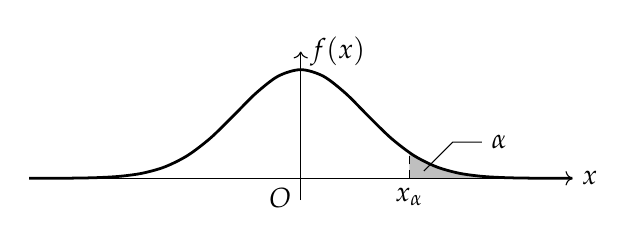
\begin{tikzpicture}[scale=2.3]
            \fill[white!75!black,domain=0.6:1.5,smooth](0.6,0)-- plot (\x,{0.6*exp(-(\x)^2*4)});
            \draw[->](-1.5,0)--(0,0)node[below left]{$O$}--(1.5,0) node[right]{$x$};
            \draw[->](0,-0.12)--(0,0.7) node[right]{$f(x)$};
            \draw[densely dashed] (0.6,0)node[below]{$x_\alpha$}--(0.6,0.144);
            %\draw[densely dashed] (0,0.14)node[left]{$\varepsilon$}--(1,0.14);
            \draw [color=black,line width=1pt,domain=-1.5:1.5,smooth] plot (\x,{0.6*exp(-(\x)^2*4)});
            \draw (0.68,0.04)--(0.84,0.20)--(1.0,0.2)node[right]{$\alpha$};
        \end{tikzpicture}
   
    \quad 通常,对于上$\alpha$分位数,
    
    \quad\qquad 标准正态分布的记作$z_\alpha,$
    
    \quad\qquad $\chi^2(n)$分布的记作$\chi^2_\alpha(n),$
    
    \quad\qquad $t(n)$分布的记作$t_\alpha(n),$
    
    \quad\qquad $F(n_1,n_2)$分布的记作$F_\alpha(n_1,n_2)$.
\end{multicols}
    \tcbline
    \paragraph{双侧$\alpha$分位数}设$X$是对称分布(密度函数是偶函数)的连续性随机变量,若$\alpha\in(0,1),\ T_\alpha\in\mathbb{R}$满足$P\{|X|>T_\alpha\}=\alpha$,则称$T_\alpha$为$X$的双侧$\alpha$分位数.
\end{tcolorbox}

\begin{tcolorbox}[colframe=green!66!black,title={\subsection{$\chi^2$分布}}]
    $X=X_1^2+\cdots+X_n^2,\ X_1^2+\cdots+X_n^2\sim N(0,1)$且相互独立,则称$X$服从自由度为$n$的$\chi^2$分布,记为$X\sim\chi^2(n).$
\begin{itemizeg}
\item $E(X)=n,D(X)=2n$.
\item \textbf{可加性\ }若$X\sim\chi^2(m),Y\sim\chi^2(n)$,则$X+Y\sim\chi^2(m+n).$
\item $n=1,2$时单调递减;$n\geq 3$时先增后减,极大值点为$x=n-2$.
\item $\chi^2(2)=e\left(\frac{1}{2}\right)$.(指数分布)
\item $n$充分大时,(如$n>40),\chi_\alpha^2(n)\approx\frac{1}{2}\left(z_\alpha+\sqrt{2n-1}\right).$
\end{itemizeg}
\end{tcolorbox}

\begin{tcolorbox}[colframe=green!66!black,title={\subsection{$F$分布}}]
    $X=\frac{U/m}{V/n},\ U\sim\chi^2(m),\ V\sim\chi^2(n)\ X,Y$相互独立,则称$X$服从第一自由度为$m$,第二自由度为$n$的$F$分布,记为$X\sim F(m,n).$
    \begin{itemizeg}
        \item 若$X\sim F(m,n),$则$\frac{1}{X}\sim F(n,m);\quad F_{1-\alpha}(m,n)=\frac{1}{F_{\alpha}(n,m)}$
    \end{itemizeg}

\end{tcolorbox}

\begin{tcolorbox}[colframe=green!66!black,title={\subsection{$t$分布}}]
    $X=\frac{U}{\sqrt{V/n}},\ U\sim N(0,1),\ V\sim\chi^2(n),\ X,Y$相互独立,则称$X$服从自由度为$n$的$t$分布,记为$X\sim t(n)$.
    \begin{itemizeg}
        \item 当$n$充分大(如$n>50),t(n)$近似于$N(0,1).$
        \item $E(X)=0,D(X)=\frac{n}{n-2}$
    \end{itemizeg}
\end{tcolorbox}

\subsection{正态总体的抽样分布(小样本分布)}
\begin{tcolorbox}[colframe=blue,title={\subsubsection{单正态总体的抽样分布}}]
    若$X\sim N(\mu,\sigma^2),\ X_1,\cdots,X_n$为样本,\ $\overline{X}$和$S^2$分别为样本均值和样本方差(修正后),有
    $$\begin{cases}\stress{U=\frac{\overline{X}-\mu}{\sigma/\sqrt{n}}\sim N(0,1)}\\
        \stressbo{\begin{aligned}&\frac{(n-1)S^2}{\sigma^2}\sim\chi^2(n-1)\\&(\mu\text{已知时用于推断}\sigma^2)\end{aligned}}\\
    \stress{\overline{X}\text{(或}U\text{)与}S^2\text{相互独立}}\end{cases}\Longrightarrow
    \stressbo{\begin{aligned}&T=\frac{U}{S}\sigma=\frac{\overline{X}-\mu}{S/\sqrt{n}}\sim t(n-1).\\&(\sigma^2\text{已知时用于推断}\mu)\end{aligned}}$$
\end{tcolorbox}

\begin{tcolorbox}[colframe=blue,title={\subsubsection{双正态总体的抽样分布}}]
    若$X\sim N(\mu_1,\sigma_1^2),\ Y\sim N(\mu_2,\sigma_2^2),\ X_1,\cdots,X_{n_1}$与$Y_1,\cdots,Y_{n_2}$为样本,\ $\overline{X},\overline{Y}$和$S_1^2,S_2^2$分别为样本均值和样本方差(修正后),有
    $$\!\!\begin{cases}
    \stress{U=\frac{(\overline{X}-\overline{Y})-(\mu_1,\mu_2)}{\displaystyle\sqrt{\frac{\sigma_1^2}{n_1}+\frac{\sigma_2^2}{n_2}}}\sim N(0,1)}\\
    \stressbo{\begin{aligned}&F=\frac{S_1^2/\sigma_1^2}{S_2^2/\sigma_2^2}\sim F(n_1-1,n_2-1)\\&(\mu_1-\mu_2\text{已知时用于推断}\frac{\sigma_1^2}{\sigma_2^2})\end{aligned}}\\
    {U\text{与}F\text{相互独立}}\\
    \text{设加权平均}S^2=\frac{(n_1-1)S_1^2+(n_2-1)S_2^2}{n_1+n_2-2}
    \end{cases}\!\!\!\!\!\!\!\Longrightarrow
    \stressbo{\begin{aligned}&\text{当}\sigma_1=\sigma_2=\sigma,\\&T=\frac{U}{S}\sigma=\frac{(\overline{X}-\overline{Y})-(\mu_1,\mu_2)}{\displaystyle S\sqrt{\frac{1}{n_1}+\frac{1}{n_2}}}\\&\qquad\qquad\qquad\sim t(n_1+n_2-2).\\&(\frac{\sigma_1^2}{\sigma_2^2}\text{已知时用于推断}\mu_1-\mu_2)\end{aligned}}$$

\end{tcolorbox}

\begin{tcolorbox}[colframe=blue,title={\subsection{一般总体的抽样分布的极限分布*}}]
    若$X_1,\cdots,X_n$为总体$X$的样本,\ $\overline{X}$和$S^2$分别为样本均值和样本方差(修正后),设$E(X)=\mu,D(X)=\sigma^2,$有
    $$\stress{\begin{aligned}U_n=\frac{\overline{X}-\mu}{\sigma/\sqrt{n}}\overset{L}\rightarrow N(0,1)\quad(\sigma^2\text{{\bf 已知}时用于推断}\mu)\\
    T_n=\frac{\overline{X}-\mu}{S/\sqrt{n}}\overset{L}\rightarrow N(0,1)\quad(\sigma^2\text{{\bf 未知}时用于推断}\mu)\end{aligned}}$$
    
\end{tcolorbox}

\section{参数估计}

\subsection{点估计}
\paragraph{估计}$\hat{\theta}(X_1,\cdots,X_n)$为参数$\theta$的{\bf 估计量}$,\hat{\theta}(x_1,\cdots,x_n)$为参数$\theta$的{\bf 估计值},二者统称为{\bf 估计}.

\subsubsection{矩估计法(ME法)}

\begin{tcolorbox}[colframe=green!66!black]

\noindent 设总体$X$的分布依赖于参数$\theta=(\theta_1,\cdots,\theta_m),\ X_1,\cdots,X_n$是样本,估计参数$\theta$的过程如下:

\paragraph{Step1}由于各阶矩是参数的函数, 故可以列出方程组:
$$\begin{cases}
\alpha_1=E(X)=g_{1}\left(\theta_{1}, \cdots, \theta_{m}\right), \\
\alpha_2=E(X^2)=g_{2}\left(\theta_{1}, \cdots, \theta_{m}\right), \\
\quad \vdots  \\
\alpha_m=E(X^m)=g_{m}\left(\theta_{1}, \cdots, \theta_{m}\right).
\end{cases}
\text{一般情况下可解得}
\begin{cases}
\theta_{1} =h_{1}\left(\alpha_{1}, \cdots, \alpha_{m}\right) \\
\theta_{2} =h_{1}\left(\alpha_{2}, \cdots, \alpha_{m}\right) \\
\quad \vdots  \\
\theta_{m} =h_{m}\left(\alpha_{1}, \cdots, \alpha_{m}\right).
\end{cases}$$
注:有时会出现某一个方程(通常是期望的方程)是恒等方程,则需要把$m+1$阶矩的方程也列出,才能解出方程.(有效方程个数=未知参数个数)

\paragraph{Step2}计算
$$\stress{\begin{cases}
    A_{1}=\frac{1}{n}\sum_{i=1}^nX_i\\
    \quad\vdots\\
    A_{m}=\frac{1}{n}\sum_{i=1}^nX_i^m    
\end{cases}}
\text{或}
\stress{\begin{cases}
    a_{1}=\frac{1}{n}\sum_{i=1}^nx_i\\
    \quad\vdots\\
    a_{m}=\frac{1}{n}\sum_{i=1}^nx_i^m    
\end{cases}}$$

$\stress{\text{再用}A_{1},\cdots,A_{m}\text{或}a_{1},\cdots,a_{m}\text{代替上式中的}\alpha_1,\cdots,\alpha_m}$,得到\textbf{矩估计量}或\textbf{矩估计值}
$$\begin{cases}
\hat\theta_1=h_1(A_1, \cdots, A_m) \\
\quad \vdots  \\
\hat\theta_m=h_m(A_1, \cdots, A_m) .
\end{cases}
\text{或}
\begin{cases}
    \hat\theta_1=h_1(a_1,\cdots,a_m) \\
    \quad \vdots  \\
    \hat\theta_m=h_m(a_1,\cdots,a_m) .
\end{cases}$$
    
\end{tcolorbox}

\newpage

\begin{tcolorbox}[colframe=green!66!black,breakable,title=\subsubsection{最大似然估计法(MLE法)}]
\paragraph{Step 1}\
\paragraph{$1^\circ$离散型}若总体$X$属离散型,其分布律$P\{X=x\}=p(x;\theta_1,\cdots,\theta_m),\theta_i\in\Theta_i$的形式已知\Big(如$B(n,p),\text{未知参数}\theta_1=n,\theta_2=p$\Big),则事件$\{X_{1}=x_{1}, X_{2}=x_{2}, \cdots, X_{n}=x_{n}\}$ 发生的概率为
$$\stress{L(x_{1}, x_{2}, \cdots, x_{n} ; \theta_1,\cdots,\theta_m)=\prod_{i=1}^{n} p(x_{i} ; \theta_1,\cdots,\theta_m).}$$

\paragraph{$2^\circ$连续型}若总体$X$属离散型,其密度函数$f\{X=x\}=f(x;\theta_1,\cdots,\theta_m),\theta_i\in\Theta_i$的形式已知,可设
$$\stress{L(x_{1}, x_{2}, \cdots, x_{n} ; \theta_1,\cdots,\theta_m)=\prod_{i=1}^{n} f(x_{i} ; \theta_1,\cdots,\theta_m).}$$


\tcbline
\paragraph{Step 2}\ \\
取 $\hat{\theta}_1,\cdots,\hat{\theta}_m$ 使
$$\stress{L(x_{1}, x_{2}, \cdots, x_{n} ;\hat{\theta}_1,\cdots,\hat{\theta}_m)=\max_{\theta_i\in \Theta_i} L(x_{1}, x_{2}, \cdots, x_{n} ; \theta_1,\cdots,\theta_m).}$$
这样得到的 $\hat\theta_i$ 与样本值 $x_{1}, x_{2}, \cdots, x_{n}$ 有关,常记为$\hat{\theta}_i(x_{1}, x_{2}, \cdots, x_{n})$, 称为参数$\theta_i$的\textbf{最大似然估计值},相应的统计量 $\hat{\theta}_i(X_{1}, X_{2}, \cdots, X_{n})$ 称为参数 $\theta_i$ 的\textbf{最大似然估计量}.\\

\begin{tcolorbox}[colframe=white!60!black,title=Tips]
    连续型时,\ {\bf Step 2}通常是一个极值问题,可以转化为求解以下方程
    $$\stress{\frac{\mathrm{d}}{\mathrm{d} \theta_i} L(\theta_1,\cdots,\theta_m)=0,}$$
    若$L>0$,有时$L(\theta_1,\cdots,\theta_m)$的对数更容易求导,则可转化为\textbf{对数似然方程},即
    $$\stress{\frac{\mathrm{d}}{\mathrm{d}\theta_i} \ln\Big(L(\theta_1,\cdots,\theta_m)\Big)=0.}$$
    注: 并不是所有连续型都可以通过以上两条方程解出极值点,有时还要考虑定义域端点是否为最大值点.
\end{tcolorbox}
\end{tcolorbox}

\newpage
\subsection{估计量的评选标准}
\begin{tcolorbox}[colframe=blue,title={\subsubsection{无偏性}}]
设$\hat\theta=\hat\theta(X_1,\cdots,X_n)$是参数$\theta$的估计量,若$\stress{E(\hat\theta)=\theta}$,则称$\hat\theta$为$\theta$的\textbf{无偏估计}.
\tcbline
若$\lim_{n\rightarrow\infty}E(\hat\theta)=\theta$,则称$\hat\theta$为$\theta$的\textbf{渐进无偏估计}.
\end{tcolorbox}

\begin{tcolorbox}[colframe=blue,title={\subsubsection{有效性}}]
设$\hat\theta_1$和$\hat\theta_2$都是参数$\theta$的\textbf{无偏估计量}$\forall\theta\in\Theta$,都有$\stress{D(\hat\theta_1)\leq D(\hat\theta_1)}$,则一般情况下可称$\hat\theta_1$\textbf{较}$\hat\theta_2$\textbf{有效}.
\tcbline
设$\hat\theta_0$是参数$\theta$的\textbf{无偏估计量},若对$\forall\theta$的无偏估计量$\hat\theta$,有$D(\hat\theta_0)\leq D(\hat\theta)$,则称$\hat\theta_0$为$\theta$的\textbf{最有效无偏估计}.
\end{tcolorbox}

\begin{tcolorbox}[colframe=blue,title={\subsubsection{相合性}}]
若$\hat\theta\overset{P}{\rightarrow}\theta$,即对$\forall\varepsilon>0,\lim_{n\rightarrow\infty}P\{|\hat\theta-\theta|<\varepsilon\}=1$,则称$\hat\theta$为$\theta$的(弱){\bf 相合估计}.
\tcbline
若$\lim_{n\rightarrow\infty}P\{\hat\theta=\theta\}=1$,则称$\hat\theta$为$\theta$的强相合估计.
\end{tcolorbox}

\end{document}